\documentclass[a4paper,12pt]{article}

\usepackage[spanish]{babel}
\usepackage[utf8]{inputenc}
\usepackage[T1]{fontenc}

%% Sets page size and margins
\usepackage[a4paper,margin=1in,marginparwidth=1in]{geometry}

%% Useful packages
\usepackage{amsmath}
\usepackage{graphicx}
\usepackage[colorinlistoftodos]{todonotes}
\usepackage[colorlinks=true, allcolors=blue]{hyperref}
\usepackage{caption}
\usepackage{subcaption}
\usepackage{sectsty}
\usepackage{float}
\usepackage{titling} 
\usepackage{blindtext}
\usepackage[colorinlistoftodos]{todonotes}
\usepackage{xcolor}
\usepackage{textcomp}
\usepackage{hyperref}
\usepackage{fancyhdr}
\usepackage[style=ieee]{biblatex}
\usepackage{csquotes}
\usepackage{siunitx}
\usepackage{wrapfig}

\addbibresource{references.bib}
\definecolor{darkgreen}{rgb}{0.0, 0.4, 0.0}
\setlength{\headheight}{16pt}

\pagestyle{fancy}
\fancyhf{}
\rhead{Robótica}
\lhead{Manipulador \emph{{\textmu}Arm}}
\cfoot{\thepage}

%%%%%%%% DOCUMENT %%%%%%%%
\begin{document}

%%%% Title Page
\begin{titlepage}

    \newcommand{\HRule}{\rule{\linewidth}{0.5mm}}
    \center

    % University
    \textsc{\LARGE Universidad Politécnica de Madrid}\\[1cm]

    % Document info
    \textsc{\Large Robótica}\\[0.2cm]
    \textsc{\large \textit{MANIPULADORES}}\\[1cm]
    \HRule \\[0.8cm]
    { \huge \bfseries Estudio del manipulador \textit{{\textmu}Arm}}\\[0.7cm]
    \HRule \\[2cm]
    \large
    \emph{Autores:}\\
    Javier Alonso Silva - \href{mailto:javier.asilva@alumnos.upm.es}{javier.asilva@alumnos.upm.es}

    Roberto Álvarez Garrido - \href{mailto:roberto.alvarezg@alumnos.upm.es}{roberto.alvarezg@alumnos.upm.es}

    José Alejandro Moya Blanco - \href{mailto:alejandro.moya.blanco@alumnos.upm.es}{alejandro.moya.blanco@alumnos.upm.es}\\[1.5cm]
    {\large \today}\\[2cm]
    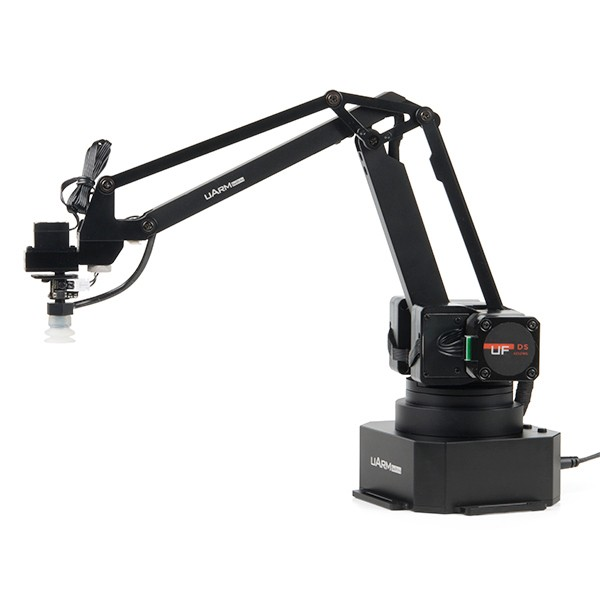
\includegraphics[width=0.5\textwidth]{images/uarm.jpg}\\[1cm]
\end{titlepage}

%%%% SECTIONS
\section*{Conocimientos previos}

Antes de ponernos a hablar sobre los resultados obtenidos en la práctica,
antes vamos a hablar sobre algunas características básicas del brazo robótico e
introducirlo brevemente.
El manipulador robótico \emph{{\textmu}Arm} es un dispositivo creado por la empresa
\href{https://www.ufactory.cc/#/}{UFACTORY} el cual cuenta con cuatro grados de libertad.
De dichos grados de libertad, tres son usados para mover el brazo robótico hasta ciertas
posiciones y, el último, para mantener el extremo del mismo paralelo al suelo.

\begin{wrapfigure}{R}{.4\textwidth}
    \begin{center}
        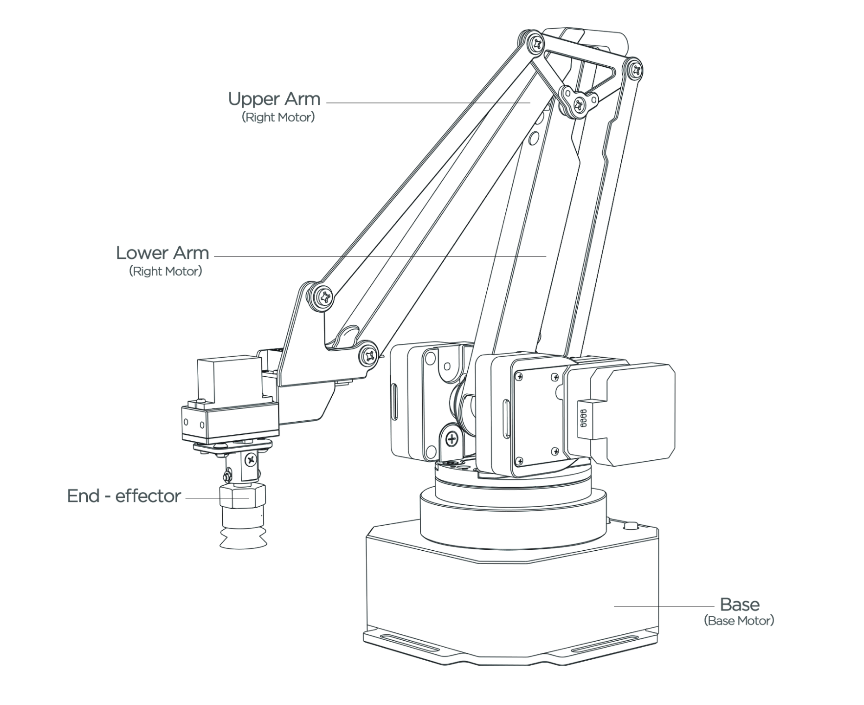
\includegraphics[width=.4\textwidth]{images/motors.png}
        \caption{zonas de actuación de los motores en el brazo \cite{developer_guide_uarm}}
        \label{fig:motors}
    \end{center}
\end{wrapfigure}

El manipulador es controlado mediante cuatro motores:

% \begin{itemize}
    El \textbf{motor de la base} el cual permite la rotación del manipulador.

    En el brazo, el \textbf{motor que está a la derecha} (ver la figura \ref{fig:motors}), 
    coordina el movimiento de la parte inferior del brazo (\textit{Lower Arm} en la figura)
    con la parte superior del mismo (\textit{Upper Arm} en la figura).

    En esta parte del manipulador, el movimiento es como el de un flexo: la parte superior
    del flexo está supeditada a la parte inferior, de manera que se mantiene de forma
    constante la altura a la que está el extremo final del mismo.

    El otro motor, localizado a la \textbf{izquierda del brazo}, se encarga de mantener la
    orientación del extremo del manipulador. De esta manera, dicho extremo
    permanecerá paralelo al suelo. Teniendo en cuenta esto, podríamos decir
    que el robot en verdad solo tiene tres grados de libertad en tanto a que no se
    controla directamente el movimiento del último grado, ya que al final se mueve
    para permanecer paralelo al suelo.

    El \textbf{motor localizado en el extremo}, con el cual se puede actuar sobre el
    elemento que esté colocado allí. Por ejemplo, cuando se coloca una ventosa
    permite rotarla o, cuando se coloca la pinza, el movimiento del motor permite
    abrirla o cerrarla.

    Para este estudio, este último motor se descartará, ya que no afecta a las
    posiciones accesibles por el robot.
% \end{itemize}

\begin{table}[ht]
    \centering
    \begin{tabular}{||c | c||}
        \hline
        \textit{Motor} & \textit{Rango de trabajo} \\ [0.5ex]
        \hline\hline
        Base & $\ang{0} \sim \ang{180}$ \\
        \hline
        Derecho & $\ang{0} \sim \ang{130}$ \\
        \hline
        Izquierdo & $\ang{0} \sim \ang{106}$ \\
        \hline
        Extremo & $\ang{0} \sim \ang{180}$ \\ [1ex]
        \hline
    \end{tabular}
    \caption{ángulo de giro de los motores}
\end{table}

\begin{figure}[H]
    \centering
    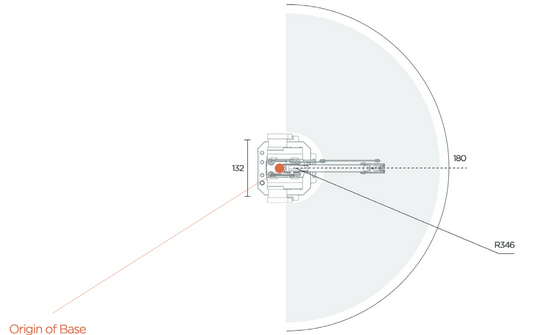
\includegraphics[height=7cm]{images/range.png}
    \caption{rango del manipulador \emph{{\textmu}Arm} \cite{user_manual_uarm}}
    \label{fig:range}
\end{figure}

Toda la información relativa al desarrollo del proyecto puede ser encontrada en
\href{https://github.com/UPM-Robotics/uarm}{GitHub - UPM Robotics} \cite{noauthor_upm-robotics/uarm_2019}. Allí están detallados
los distintos hitos a conseguir así como más información sobre el robot.

Además, está detallada la siguiente bibliografía:
\begin{itemize}
    \item \href{https://github.com/UPM-Robotics/uarm/blob/master/docs/robot-information/uArm%20pro%20User%20Manual%20v1.1.0.pdf}{Manual de usuario}
    \item \href{https://github.com/UPM-Robotics/uarm/blob/master/docs/robot-information/uArm-Swift-Specifications-171012.pdf}{Especificaciones}
    \item \href{https://github.com/UPM-Robotics/uarm/blob/master/docs/robot-information/uArm%20Swift%20Pro_Developer%20Guide%20v1.0.6.pdf}{Guía del desarrollador}
    \item \href{https://github.com/UPM-Robotics/uarm/blob/master/docs/robot-information/uArm_Swift_Pro_3D_20180620.STEP}{Modelo en 3D}
    \item \href{https://www.ufactory.cc/#/en/}{Web de UFACTORY}
    \item \href{https://www.ufactory.cc/#/en/support/technology}{Soporte de UFACTORY}
\end{itemize}

\newpage
\section{Configuración geométrica}

En esta sección vamos a describir la configuración geométrica del brazo robótico. La
configuración que obtuvimos fue la siguiente:
\begin{figure}[H]
    \begin{minipage}{.48\linewidth}
        \centering
        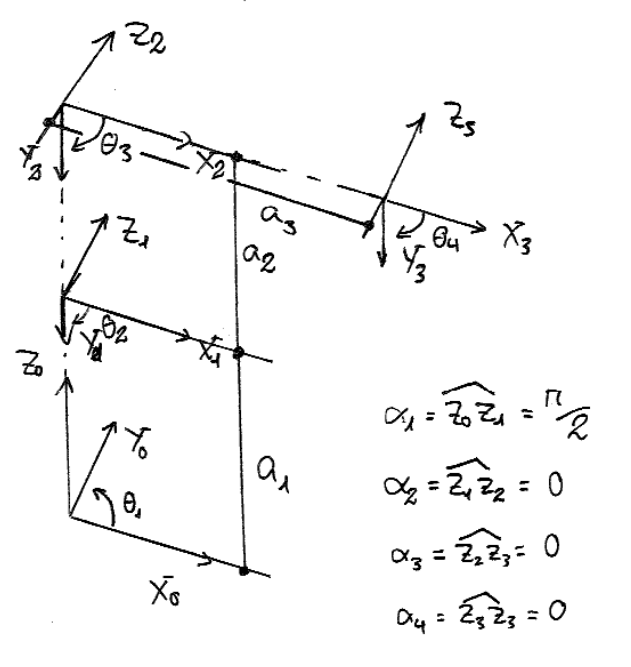
\includegraphics[width=.7\linewidth]{images/geometric_configuration.png}
        \caption{configuración geométrica del robot}
        \label{fig:robot_config}
    \end{minipage}\hfill
    \begin{minipage}{.48\linewidth}
        \centering
        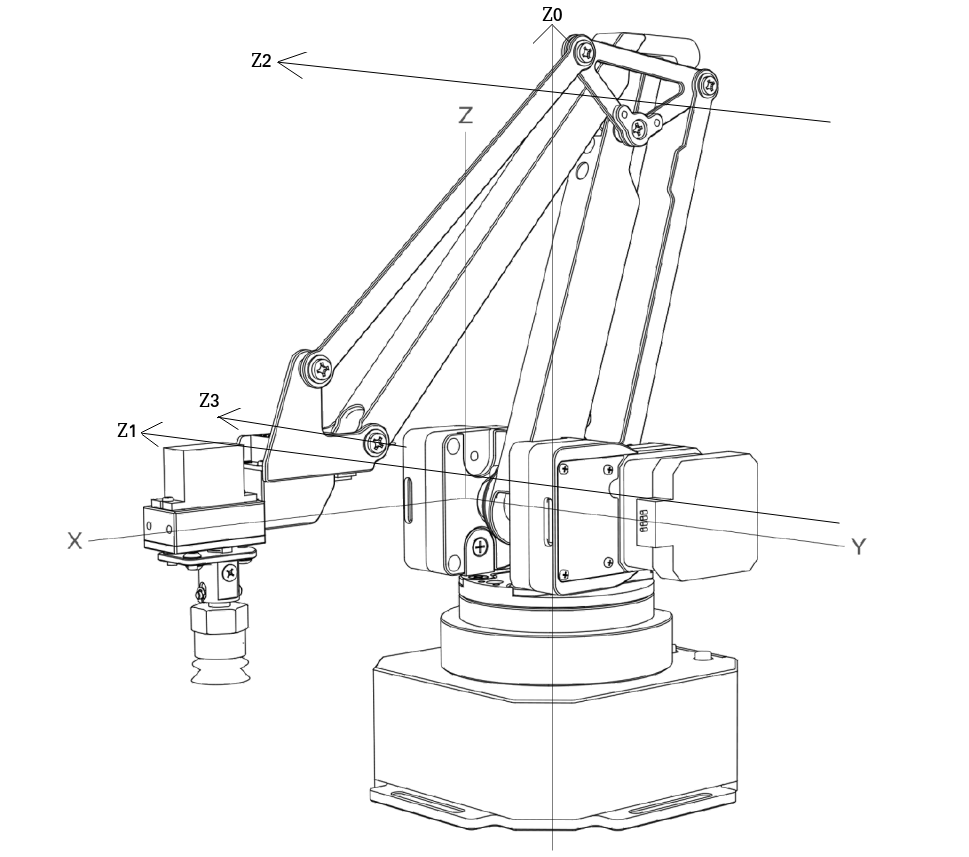
\includegraphics[width=.7\linewidth]{images/axis.png}
        \caption{los grados de libertar del brazo, representados por los diferentes $Z_i$}
        \label{fig:axis}
    \end{minipage}
\end{figure}

Usando los datos que están presentes en la documentación al desarrollador \cite{developer_guide_uarm},
pudimos obtener los siguientes datos para los $a_i$ (distancia entre ejes) del manipulador; además,
descubrimos que hay una pequeña desviación $d_i$ entre las articulaciones $\{1, 2\}$:
\begin{figure}[H]
    \centering
    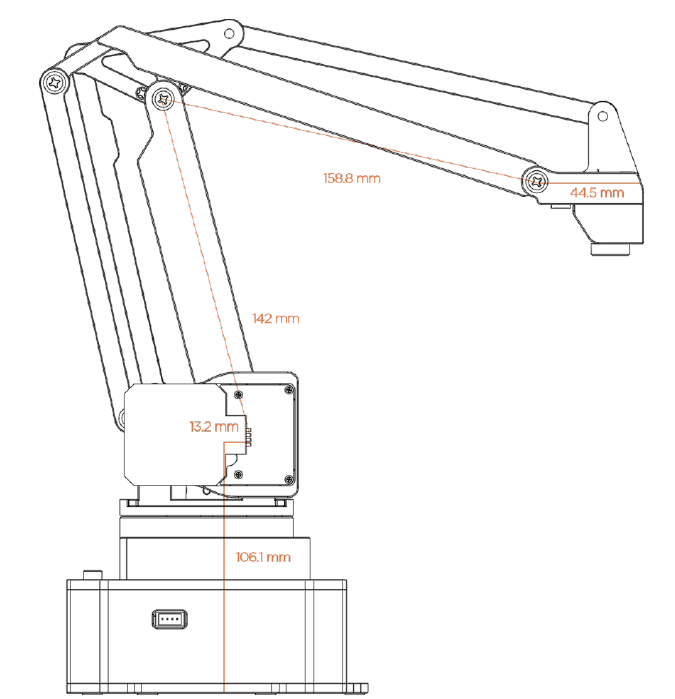
\includegraphics[height=6cm]{images/sizes.png}
    \caption{longitudes del brazo robótico \cite{developer_guide_uarm}}
    \label{fig:sizes}
\end{figure}

\begin{table}[H]
    \centering
    \begin{tabular}{|| c | c c ||}
        \hline
        $i$ & $a_i~(mm.)$ & $d_i~(mm.)$ \\ [0.5ex]
        \hline\hline
        $1$ & $106.1$ & $0$ \\
        \hline
        $2$ & $142$ & $13.2$ \\
        \hline
        $3$ & $158.8$ & $0$ \\
        \hline
        $4$ & $44.5$ & $0$ \\ [1ex]
        \hline
    \end{tabular}
    \caption{longitudes y desviaciones del manipulador}
\end{table}

De esta manera, con los datos obtenidos, obtenemos las siguientes tablas de \textit{Denavit–Hartenberg}:

\begin{table}[H]
    \parbox{.45\linewidth}{
        \centering
        \begin{tabular}{ c | c c c c }
            $i$ & $\theta_i$ & $d_i~(mm.)$ & $a_i~(mm.)$ & $\alpha_i$ \\ [0.5ex]
            \hline
            $1$ & $\theta_1$ & $0$ & $106.1$ & $-\frac{\pi}{2}$ \\
            $2$ & $\theta_2$ & $13.2$ & $142$ & $0$ \\
            $3$ & $\theta_3$ & $0$ & $158.8$ & $0$ \\
            $4$ & $\theta_4$ & $0$ & $44.5$ & $0$ \\ [1ex]
        \end{tabular}
        \caption{tabla de \textit{Denavit–Hartenberg}}
    }
    \hfill
    \parbox{.45\linewidth}{
        \centering
        \begin{tabular}{ c | c c c c }
            $i$ & $\theta_i$ & $d_i~(mm.)$ & $a_i~(mm.)$ & $\alpha_i$ \\ [0.5ex]
            \hline
            $1$ & $\theta_1$ & $0$ & $a_1$ & $-\frac{\pi}{2}$ \\
            $2$ & $\theta_2$ & $13.2$ & $a_2$ & $0$ \\
            $3$ & $\theta_3$ & $0$ & $a_3$ & $0$ \\
            $4$ & $\theta_4$ & $0$ & $a_4$ & $0$ \\ [1ex]
        \end{tabular}
        \caption{tabla de \textit{Denavit–Hartenberg} en función de $a_i$}
    }
\end{table}

\newpage
\printbibliography

\end{document}